\documentclass{article}
\usepackage{graphicx} % Required for inserting images
\usepackage[a4paper,left=2.5cm,right=2.5cm,top=2cm,bottom=2cm]{geometry}
\usepackage{minted}
\usepackage{lipsum} % Package for generating dummy text

\usepackage{graphicx}
\usepackage{subcaption} % for subfigures
\usepackage{mdframed}



\setminted{fontsize=\small, baselinestretch=1}


\title{Decentralized Finance \\
  \large {A Summary}
\author{Sarah Kuhn}
\date{April 2024}
}

\begin{document}
\maketitle
\thispagestyle{empty} % Remove page number from the first page

\newpage
\pagenumbering{arabic} % Start page numbering from 1
\setcounter{page}{1} % Set page counter to 1

\section{Finance Basics}
Let's start with some basics of finance to understand why financial markets are so important. Financial markets are like giant networks where people and companies can invest money, raise funds, and manage risks. They  determine the prices of things like stocks, bonds, currencies, and also more exotic investments. These markets are essential for our economy because they allow  businesses to grow, people to invest their savings, and governments to manage their budgets more easily.

\subsection{Financial Markets: Underlying assumptions} 

Before we dive deeper into financial markets and their impact on our economy, let's first fix the foundation and basic assumptions upon which we build our hold study of finanical markets on:  Financial markets are incredibly complex, as they are influenced by the decisions of billions of individuals. To tackle this complexity, we simplify things by making certain assumptions like we often do. One base assumption we make is that people act rationally and secondly, that markets operate efficiently. This simplification helps us and professional economists to create models and theories which explain what we see happening in the markets and even make predictions about future trends. The assumptions described in the next subsection can be seen as the foundational building blocks to even make statements about financial markets and financial systems in general.

\begin{itemize}
    \item \textbf{Rational Expectations}

Definition: Rational expectations suggest that individuals form expectations about the future by considering all the information available to them at the current time point. They use these expectations to guide their decision-making process. These expectations are called "rational" because they align with the information known at the time.

In Financial Markets: Rational expectations imply that investors take into account all available information, such as historical prices, economic facts, and obviously news, when forecasting future asset prices. This implies that asset prices reflect the collective opinion and expectations of investors. It also suggests that individuals will not consistently make errors in predicting the future, including risks. Overall this assumptions leads to markets being considered efficient in the long term.

%not sure if its understandble what i mean efficient markets ?

\item \textbf{Efficient Financial Market Theory}

Definition: Efficient market theory suggests that financial markets quickly and accurately incorporate all available information into asset prices. So "asset prices represent the best possible estimates of the risk attached to them" (from lecture slide). Thus the risk from a financial market or just an investment can be inferred through mathematical analysis.
\end{itemize}

\subsection{Role of Financial Markets} 
Financial markets play a key role in our economy by fulfilling several functions:
\begin{itemize}
    \item \textbf{Raising Capital}:
    We can think of financial markets as vast platforms for fundraising. Companies and governments turn to these markets to seek investments from individuals and institutions. They can do this by selling shares of their company or issuing bonds to raise money. This "flow" of capital helps them fund their operations and start financing  new projects.
    %can we say that in english ?
    
    \item \textbf{Economic signaling}: We could also call this "setting fair prices": In financial markets, prices of assets like stocks and bonds are determined by how many people want to buy or sell them. Its often refered to as the demand and the supply. This process helps investors know if they're paying a reasonable price for their investments.
    
    \item \textbf{Ease of trading}: The financial market provides a convenient platform for individuals to trade assets such as stocks and bonds whenever they need it. This flexibility is essential as it enables investors to quickly adjust their portfolios in reaction to changing conditions. It is often stated that financial markets offer liquidity to investors, as they ensure easy access to funds when needed.
    
    \item \textbf{Risk management}: In the financial market, individuals have access to tools to "secure" their investments from unexpected events that could lead to losses, such as sudden market fluctuations or in general unexpected bad events. This strategies/tools are summarized as "hedging against risk." By employing instruments like options, futures, or swaps, investors can shield themselves from  movements that may affect the value of their assets negatively. Essentially, this involves investors gambeling ? on the possibility of asset value loss . If this scenario occurs, the investor profit as they accurately predicted the loss. Another method of risk management is diversification, which involves spreading investments across different asset classes and categories (e.g., geographical or industry-based) to reduce overall risk. This strategy works as one loss incurred in one investment can be compensated by gains in others, which leads to a more balanced investing approach.
    
     \item \textbf{Economic growth}: Financial markets play a main role in fostering economic growth by providing capital to various economic actors such as companies and governments. This provision?  of capital enables these entities to expand their operations and take on on new initiatives, such as investing in infrastructure projects. This can lead to the creation of more job opportunities and contribute to overall economic prosperity.
\end{itemize}

\subsection{Stakeholders in Financial Markets} 
In the previous section, we examined the role of financial markets within an economy. Now, let's dive deeper into the key participants, often referred to as stakeholders, in the world of finance. A stakeholder stands for any individual or group capable of influencing or being influenced by the actions and consequences of financial markets. This "umbrella term" summarizes various actors such as:

\begin{itemize}
\item \textbf{Investors}:
Investors are individuals or organizations that supply funds to companies and governments in exchange for ownership(f.eg through buying a stock you are basically "owner" of a fraction of the company) or the promises of future returns. They come in various forms, from individual investors managing their personal portfolios to institutional investors like pension funds, which pool money from multiple investors and then invest it on their behalf. Investors typically acquire financial assets such as stocks, bonds, or also ETF, aiming to grow their wealth over time through positive returns on their assets. You can also think of it like the investors lend their money to companies with the belief that in the future the company will have a return because they used the money profitable. And then as an investors you will get parts of this big win because you were so nice and provided liquidity through lending your money.

\item \textbf{Issuers}:
Issuers, as their name implies, are entities that issue financial instruments. They are organizations such as companies or governments, which provide financial products to investors to raise capital for diverse purposes. By offering financial instruments like stocks or bonds, issuers gain access to funds, thereby gain liquidity. They can utilize these funds for various projects, such as financing projects, expanding operations, or repaying their existing debts. For instance, when you purchase a company's stock as an investor, we refer to the company as the issuer of the stock.

\item \textbf{Intermediaries}:
Intermediaries act as "the man in the middle", bridging the gap between investors and issuers by making the trading of financial assets in the market easier. Think of them as the middlemen who coordinates the process of investing. Without intermediaries, investors would need to individually approach companies to discuss investment options, which wouldn't be  efficient nor scalable. Hence, entities like banks and stock exchanges step in to provide a platform and also information about the services and the execution of the serivce itself. They are the main players in matching buyers with sellers and ensuring correct transactions. In essence, intermediaries are vital for the correct and smooth functioning of financial markets. They massivly contribute to market efficiency and accessibility.

\item \textbf{Regulators}:
Regulators, as their name suggests, are tasked with overseeing and regulating the financial markets to ensure their integrity, fairness, and stability. They establish and enforce rules, also known as regulations and standards, fixing on how interactions of market participants such as investors, issuers, and intermediaries should ahppen. The primary responsibility of regulators is to monitor market activities to maintain trust in the markets and ensure the needed transparency. They also have a understanding of the connections and interdependencies among financial institutions. Because of this overseeing position, regulators play a crucial role in preventing systemic risks that could lead to a collapse of the entire financial market, as has occurred in the past f.eg in 2008.

\item \textbf{Market data providers}:
Market data providers are organizations responsible for collecting and processing information about financial markets for participants. They gather data on asset prices, trading volumes etc. Hence they offer valuable insights for investors,  issuers and even regulators. Much of our investment decisions are based on the data provided by these market data providers. We all agree that access to timely and especially accurate market data is essential to make informed decisions on the finincial market.
\end{itemize}

\subsection{Risk of Financial Markets}
So we have seen what financial markets bring to the economy and that they are like a bustling marketplace where people buy and sell all sorts of financial products, like stocks and bonds. But with all the e potential for profit also comes a fair share of risk. In this section, we'll take a closer look at what financial risk means and how the rise of DeFi is promising to change the game.

Having explored the contributions of financial markets to the economy in the previous chaptre, we know understand them as places where individuals engage in buying and selling various financial products, such as stocks and bonds. We can also say they are the place where demand and supply meet. However, alongside the potential for profit, there also exists a considerable amount of risk. In this section, we will look at financial risks. With this we will also see where the notion of DeFi stems from and how the rise of DeFi is promising to change the game.
\subsection{Market Vulnerability} 
Financial markets are exposed to a variety of diffrent factors, each carrying its own unique risks.
\begin{itemize}
    \item \textbf{Systemic risk}: Participating in financial markets naturally exposes the actors to systemic risk, which impacts the entire system rather than an individually actor. These risks come from various sources, such as political events or regulatory changes, and have an effects across the entire financial system.
    \item \textbf{Market risk}:  These losses exist due to changes occurring directly within the market, such as fluctuations in exchange rates or declines in interest rates.
     \item \textbf{Credit risk}:  Credit risks refer the the potential loss when the borrowers creditworthiness changed and he might be in financial distress and thus not able to repay the credit.
    \item \textbf{Operational risk}:  This risk describes the potential of internal operations and intermediaries failing. Examples would be an error in the system or a fraud.
    \item \textbf{Cyber Security Risk}: This is a rather new and upcoming risk. As financial markets use more and more technology, cyber attacks on financial institutions increase and lead to loss of sensitive data, theft and other disruptions. 
\end{itemize}


\subsection{The DeFi promise } 
In the previous section, we explored how centralized financial markets, where all transactions are routed through a central authority, pose various risk potentials. Particularly after the 2008 economic crisis, trust in such centralized financial structures sank. In November 2008, Satoshi Nakamoto released software that started Bitcoin.He promoted it as a "fully peer-to-peer system with no trusted third party." For many, this marked the birth of DeFi systems. But what exactly are the promises of DeFi?

\subsubsection{From CeFi to DeFi}

\begin{itemize}
    \item \textbf{Inclusivity}:DeFi aka Decentralized Finance, aims to offer financial services to individuals all over the world, including those who lack access to traditional banking services.
    \item \textbf{Innovation}: DeFi platforms are mostly open-source and allow developers to create and deploy financial applications without needing approval from centralized institutions.
    \item \textbf{Reduced Cost}: In DeFi, intermediaries are often replaced by automated processes, such as smart contracts which we will encounter later on. As a consequence DeFi has the potential to offer lower costs compared to traditional financial services.
    \item \textbf{Transparency}: Transparency is a key concept in DeFi. Technologies like the blockchain offer transparency by allowing every user to view and trace each transaction and activly engage wherever in the system. This transparency enhances or at least aims to enhance trust in the financial system for many individuals.
    \item \textbf{Financial Empowerment}: This is a key promise of DeFi: It promises to empower individuals by guaranteing them greater control and access over their own assets. In DeFi, users often possess a private key, enabling them to directly to engage in financial exchanges and transactions without needing any traditional intermediaries. But this also brings its own risk.
\end{itemize}


\subsection{Extra: Smart Contract} 
This section will introduce smart contracts. While they haven't been covered in the course yet, I believe it's important to provide an introduction now, as the concept of programmable money is fundamental to DeFi. ll in all, smart contracts enable the automation of financial processes without the involvement of third parties, as in centralized finance (CeFi) systems.\\

Smart contracts are  self-executing contracts with conditions and rules directly encoded into their code. They are applications deployed directly on a blockchain, executing automatically when predefined conditions coded within them are fulfilled. Once deployed, a smart contract's code cannot be altered, which leads to a certain inflexibility but with it also a high level of trust for the transaction parties. By eliminating intermediaries, smart contracts stand for autonomy, which is a very important word in DeFi and also reduces  the risk of fraud or manipulation. And as we eliminate a third party in the middle coordinating the transactions smart contracts allow us to reduce both time and cost which are usually associated with traditional contract executions.

So, what exactly is inside a smart contract then? In basic words: It serves as an agreement between two parties and handles transactions between them. These parties establish specific rules and encode them within the smart contract. When their defined conditions are met aka the contract is fulfilled, it autonomously executes the transaction without requiring intermediaries like banks to issue it.

\subsubsection{Example in Solidity}
Here, we'll show some basic components of a smart contract. Various programming languages are utilized for writing smart contracts, but the most used language for the Ethereum blockchain is Solidity. It's a statically-typed language with syntax like JavaScript.

\begin{minted}[linenos, xleftmargin=20pt]{solidity}
// SPDX-License-Identifier: MIT
pragma solidity ^0.8.0;

contract SimpleExampleTransaction {
    address public owner;

    // Constructor to set the owner of the contract
    constructor() {
        owner = msg.sender;
    }

    // Function to send ether from the contract to a specified receiver 
    function sendEther(address payable _recipient, uint256 _amount) public {
        require(msg.sender == owner, "Only owner can send ether");
        require(address(this).balance >= _amount, "Not enough balance in the contract");

        _recipient.transfer(_amount);
    }

    // Function to get the contract's balance
    function getBalance() public view returns (uint256) {
        return address(this).balance;
    }
}

\end{minted}
\section{Introduction to Ethereum}
\section{Oracles}
This chapter is about Oracles and their importance for a blockchain network. Oracles tackle the question on how to write data into the blockchain and keep the data up to date. One could say a lack of the blockchain technology is that a blockchain is an isolted database. Per default a blockchain cannot access real word events or just browse the internet to get the newest data, thus has no access to off-chain events. Hence another mechanism is needed that allows us to integrate relevant data on the chain.\\
\\
In the context of Ethereum an oracle refers to a trusted source of external aka off-chain information that f.eg smart contracts can use to make decisions and thus perform actions based on real-world events. Earlier we learned that smart contracts are automated contracts that will execute as soon as their encoded condition is satisfied. So often real-word data like price tables, sports score or financial market data is requested. At this point oracles then serve as a bridge between the contract on chain and the external data: Hence they fetch external data from off-chain sources, verify its authenticity and then provide this data to smart contracts on the blockchain.\\
If we wouldn't have those oracles the range of DeFi applications would be way more limited. 
For some an oracle node might still seem very abstract, so the next subsection will go into more depth about these kind of components and espeically how they are designed. It might be skipped.

\subsection{Oracle in more depth}
To me oracles first seemed very abstract and I couldn't really imagine what the structure behind such a node looked like. To start with, we can look at an simple oracle analogy. Imagine you are locked in a room, studying while having access to all the textbooks and resources you need to complete your assignments (data stored on the blockchain). However, you're not allowed to leave the room or access any information from the outside world. Now, let's say you're working on a project that requires information about the temperature outside. But since you're stuck inside the room, you can't see what's happening outside. Now the oracle is like a trusted friend who has the ability to go outside the room (access external data sources) and check the data you need for you. So your friend goes outside, checks the weather, and comes back to tell you (provides external data to the smart contract). Now based on the info provided by your friend (oracle), you make a decision about the future of your project (execute actions in the smart contract based on external data).
\\
\\
So all in all an oracle node is a piece of software/service that runs on existing computing infrastructure and interacts with external data sources to retrieve and provide data to smart contracts on the blockchain. We can kinda think of it as an application that is installed and executed on a computer/server. It is responsible for fetching the requested data from external sources like the web and then transmitting it to smart contracts on the chain. There exist multiple, actually many many, oracle nodes and each runs on dedicated servers, virtual machines or even private computers. In decentralized systems we have so called oracle networks aka oracle nodes distributed across multiple locations and operated by different participants. Collectively they then provide reliable oracle data service to smart contracts. If one as an participant provides an oracle, it mostly refers to providing the computational resource the run the piece of software, hence provide the oracle service. Anyone who wants to, can actually provide an oracle service tot  a blockchain . This means deploying software or infrastructure that retrieves, verifies and then transmits data from the external world resource to smart contracts on a blockchain. 

\subsection{Oracle Design Challenge}
Now that we know what Oracles are and why the are relevant, the questions is how do we efficiently integrate Oracles in our DeFi system and how do we design them?\\
\\
First of all, when dealing with oracles the reliability of the data they provide is crucial. If one oracle provides incorrect data, it can potentially destroy the outcome of smart contracts relying on that data. To reduce this risk various approaches to guarantee accuracy of oracle data are used. Some strategies are:\\
\\
\textbf{Multi-sourcing}: Instead of relying on a single oracle, smart contracts can fetch data from multiple independent oracles. By looking at and collecting data from multiple sources, we (i.ex the smart contracts) can afterwards use techniques such as calculating the median, the weighted averaging, or outlier detection to filter out potentially wrong or disturbing data points. In this way we reduce the risk of malicious data  and in general improve reliability of the data.\\
\\
\textbf{Majority Voting/ Consensus}: In a previous Parallel Programming course, we looked at consensus protocols, which are now relevant in the context of oracles. Consensus protocols help prevent the integration of unreliable data from an oracle into our blockchain. By comparing data provided by multiple oracles, we can determine the majority aka the consensus value. This refers to the  value they agree on or have in common, which becomes the final data we work with. While the implementation of consensus can involve simply comparing values, it often requires more complex, so called consensus algorithms.

Now that we have tackled the challenge of ensuring reliable data in our smart contracts, the next problem is how to manage fails?, whether they occur with an oracle node or withhin the source from which we want to retrieve the real-world data.
\\
This scenarios are called Oracle outages and source outages and refer to situations where the oracle service or the original data sources providing information to smart contracts become unavailable. How we handles these is important as imagine f.eg an smart contract execution gets delayed or has an incorrect outcome because of missing data. Nowadays there are some used strategies to react upon such outages:\\
\\
A possible strategy is to implement \textbf{redundancy}. This means using multiple independent Oracles or data sources, so if one becomes unavailable, the smart contract can switch to another reliable source without interruption. So even when an Oracle outage occurs the other Oracles can take over and thus ensure continuity and reliability of the data.
The same idea holds for an source outage. Instead of having one external source with the relevant information, we fetch it from different websites, thus reducing the impact of an outage of a single website. Another possible approach is to implement default values into the smart contract or make them use or historical/the previous used data. This strategy is called the \textbf{"Fallback procedure"} and is an effective way to handle outages. As the name suggest we fallback to old data values.\\
\\
As we see there are a lot of questions and also options to consider when planning on how to design and implement an Oracle network, further challenges the reader may think about are:
\\
insert question from the slides still but was to lazy at some point bc didtn intrest me hahah
\\

\subsection{On-Chain Oracles}
An additionally design possbility or rather functionality we will look at are on-chain Oracles. It might sound contradictory as Oracles are mostly used to retrieve external off-chain data but obviously one can also make use of them to determine the price of on-chain assets. Intuitively it makes sense as there most likely also exists smart contracts that need data from the blockchain. On-chain oracles are the ones providing that information to the smart contracts. So on-chain oracles are a type of oracle service where the data retrieval, processing, and transmission occur entirely within the blockchain. They don't interact with external data sources like traditional oracles but retrieve data directly from within the chain. The fetched data may include information stored in other smart contracts, blockchain transactions or other "state variables" from within the blockchain network. On-chain oracles can then also pre-process the data before transmitting them to the smart contracts. f. eg the can aggregate data from multiple sources, apply maths formulas or even algorithms. Finally they then transmit the gained data directly to smart contracts within the same (!) blockchain network. This transmission occurs through blockchain transactions or function calls between smart contracts. On-chain Oracles are especially useful for getting prices for DeFi applications, where the smart contracts require real-time access to f.eg cryptocurrency prices. But one has to keep in mind that on-chain oracles also bring certain risks as we will see in later chaptres (security chaptre). They f. eg can be manipulated and thus destroy the functionality of smart contracts.

\section{Censorship}

In this chapter we will look at the possibility of censorship on different layers of a blockchain and the implications it has. Censorship can be and is implemented at different layers of the blockchain. To look at that we will first recap the different layerings and see where censorsing of transaction could happen.
\subsection{Blockchain layers}
A blockchain can be imagined similar to a computer network with its different layers. Each layer responsible for different aspects of the blockchains functionality. Layers often referd to when we talk about blockchains are:\\
\\
\textbf{Network Layer}:The network layer stands for the communication and data propagation among nodes in the blockchain. It has the famous peer-to-peer communication protocols for transmitting transactions, blocks, and other network messages between nodes.\\
\\
\textbf{Consensus Layer}: The consensus layer mainly is responsible for the rules and protocols for achieving agreement among nodes on the validity and ordering of transactions in the blockchain. Different consensus mechanisms are implemented at this layer to govern how nodes reach consensus (aka agree on certain services and data) and produce new blocks.\\
\\
\textbf{Block Production}: This layer manages the process of block creation and propagation within the blockchain network. It selects the block producers and appends new blocks to the blockchain according to the consensus rules.
Smart Contract Layer: The smart contract layer enables the execution of the "programmable agreements". Smart contracts are self-executing contracts with predefined conditions and actions encoded. The stand for the automation of transactions without needing intermediaries.\\
\\
\textbf{(Decentralized) Application Layer}: The application layer contains decentralized applications built on top of the blockchain.
\\
Like with computer networks organizing the blockchain a into distinct layers brings modality and each layer contributes to the overall functionality and security of the blockchain network.


\section{Censorship at different levels}
To talk about censorship we first have a look at the definition of censorship. Censorship is know as the phenomena of suppressing or restricting certain data to be published or transmitted. In the context of DeFi we it is refereed to as the manipulation or even complete surpression of financial information like transactions regarding a decentralized platform. It is often claimed that DeFi, especially the blockchain avoids having censorship. But however there are scenarios where censorship  can still occur in various forms within the DeFi system. We distinguish between weak and strict censorship. Obviously there is no strict line defining weak and strong censorship but here are some examples which may give some intuition.
\\
\\
\textbf{Weak Censorship}: 
Imagine a mining pool selectively blocking or delaying a certain transaction. This means they repeatedly refuse to include certain transactions into a block to mine. The mining pool could decide to censor activities from certain addresses and never include the transaction stemming from there. But in weak censorship there might still be some other mining pools that process the transaction and include it in their suggested block. So the transaction can still be execute at some point in time but with some delay and inconveniences for the user.\\
\\
\textbf{Strong Censorship}: 
Strong censorship involves more effort and coordination of the whole system to suppress a transaction or even ti modify the blockchain's transaction history y f.eg. invalidating certain transactions. This sometimes happens when certain issues arise like a smart contract getting exploited or in general security issues appear. The system then "rolls back" to a state before the "bad" event occurred. Now it seems as the event has never happened. We see that strong censorship really needs consensus and coordination among the whole system while weak censorship can happen more locally.
The question now is how can we ass users avoid to be censored ?
\subsection{Censorship Resistance}
A solution attempt on the Ethereum blockchain is \textbf{Tornado Cash} . Tornado Cash is a so called mixer which allows users to make transactions more private by breaking the link between the sender and receiver blockchain addresses and "encrypting" the transaction amount. We as users can deposit ETH into the Tornado Cash's smart contract ( actually a set of smart contracts) and as we deposit money there we can choose an anonymity set. This defines our desired level of privacy, the larger the anonymity set we choose, the more private our transaction will be ( 1/ cardinally of anonymity set). Additionally a mixer allows us to only place a certain amount of ETH f.eg 1 ETH  at a time because transaction amounts are also data channels to backtrack a transaction. After depositing tornado cash will mix our transaction which means that it gets combined with other activities from the anonymity set. This the breaks the link between the sender and recipient address. Finally after the mixing we can withdraw our funds to a new address. Technically we could withdraw it from the same address but then the whole point of privacy is lost. All in all it Tornado cash and in general mixers make it more difficult for outside observers to track financial activities on the blockchain. This is useful for if you want to  protect your financial activities from analysis of other parties. I still want to mention that the use of tornado  cash doesn't necessarily provide 1oo\% privacy f.eg if you have to interact with a DeFi App to reach the mixer etc.
\begin{figure}[h]
    \centering
    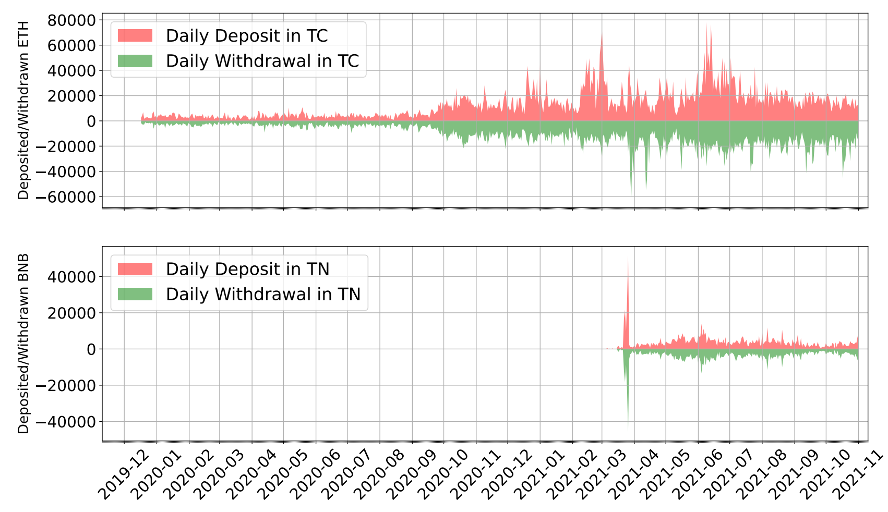
\includegraphics[width=0.5\textwidth]{tc.png} % Replace 'example-image' with the filename of your image
    \caption{Tornado Cash Interactions, \scriptsize{source: lecture 2}}
    \label{fig:image-example}
\end{figure}

\subsection{Security Implications of Censorship}
Assume a node is censoring transactions, now the questions is what does that node have to perform ? If a node doesn't just censor all of the incoming transactions, it has to go through a predefined list containing all the black-listed addresses. Thus it has to loop through this list and perform computations, check whether to censor it or not, hence has to use computational power on that transaction even though it will be drop at the end. Now an attacker could just generate a big batch of transactions an spam the node. For this transaction creation must be cheaper than transaction validation. The node then has to process this transactions and check if it should execute them. So we se that on the one hand censorship's is important to provide some legal compliance and fight against malicious users but on the other hand it is a platform for denial of service attacks and slows down transactions.
\\
\\
\textbf{Extra: Denial of Service Attacks:}\\
In this subsection we will quickly take a closer look at denial of service attacks on censoring nodes. We know that a Ethereum transaction involves different actors from validiators to miners etc. and each of those nodes can be responsible for censoring certain addresses. A DoS attack on those censoring nodes in a blockchain consist of flooding the network with transactions to overwhelm the nodes responsible for censoring transactions. So the nodes are occupied with other computations than censorship and thus leads to censorship policies getting ignored or increased  congestion in the system.

The following piece of code shows the structure of a computationally heavy transaction that could execute such a DoS attack:

\begin{figure}[h]
    \centering
    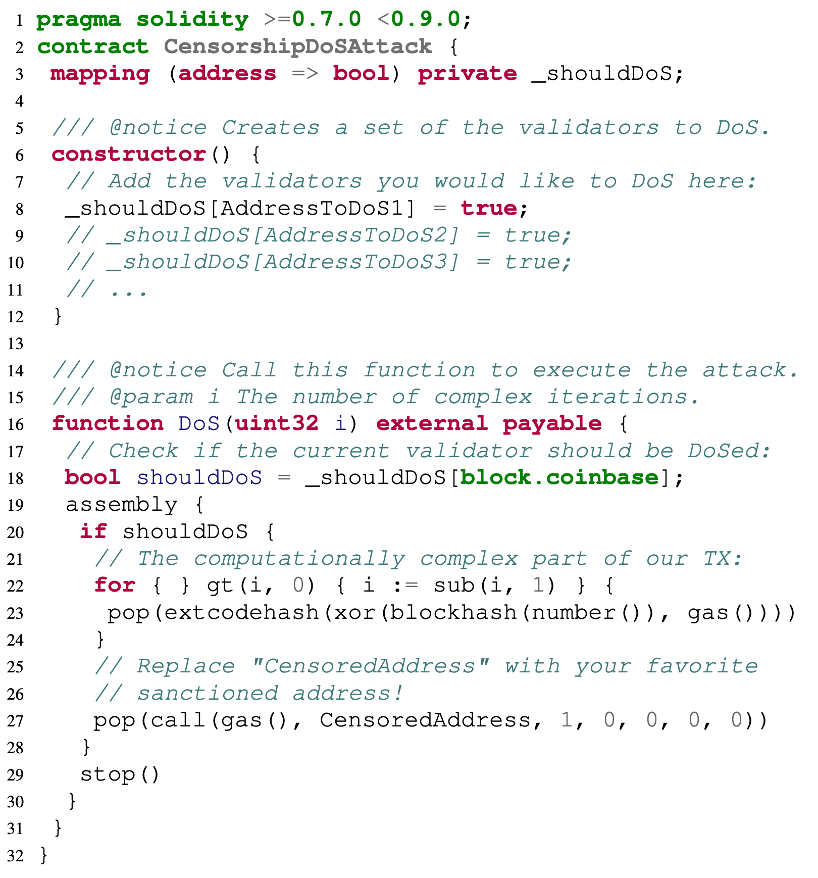
\includegraphics[width=0.5\textwidth]{dos-attack.png} 
    \caption{Example Code Of An Expensive Transaction, \scriptsize{source: lecture 2}}
    \label{fig:DoS-attack}
\end{figure}


\section{Decentralized Exchanges}
In this chapter we will look at so called DEX's, decentralized exchanges. In the finical world the exchanges are a center piece.There exist exchanges with all level of sophistication. A characteristic for a DEX is that it operates directly peer-to-peer without having a single trusted authority in the middle. But how do this exchanges operate ? How are the decentralized exchanges implemented ?

To make sure that we all are aware of why exchanges are useful and needed: Exchanges are platforms for individuals to buy, sell, and trade assets, in DEX's theses assets are mostly cryptocurrencies. In exchanges buyers and sellers get matched and overall exchanges make it easier for investors and companies to find a corresponding match.
\begin{figure}[h]
    \centering
    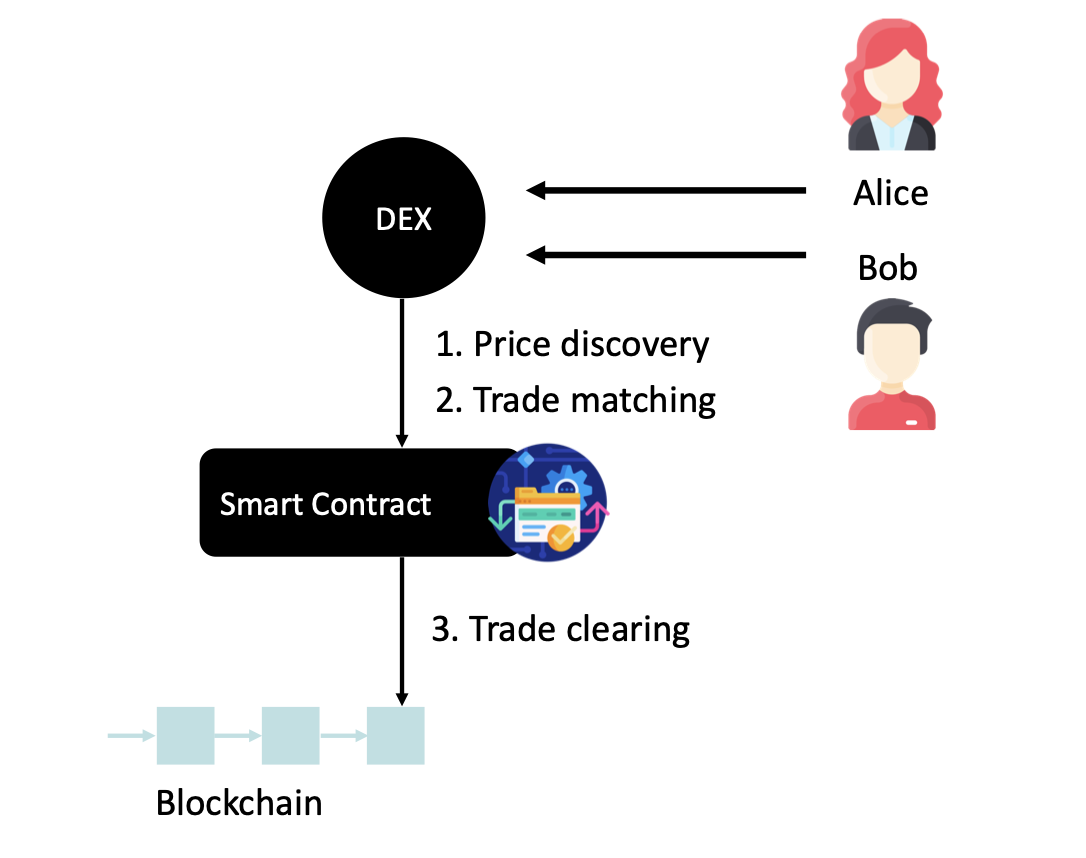
\includegraphics[width=0.5\textwidth]{Bildschirmfoto 2024-04-02 um 13.49.50.png} % Replace 'example-image' with the filename of your image
    \caption{Position of DEX, \scriptsize{source: lecture 4}}
    \label{fig:DoS-attack}
\end{figure}

What are steps that have to be done ?
\begin{itemize}
    \item {price discovery}
    \item {price matching}
    \item {actual transfer}
\end{itemize}


\subsection{Order books}
Order books are the core component of DeFi exchanges. They are an essential tool for traders to understand market liquidity and the amount of demand in the exchange. In Order book usually buy orders and sell orders are each listed on one side with corresponding information about the price and the quantity. The orders get placed by a so called market maker which gets to order request and puts them in them into the exchange system. An important characteristic of order books is the order depth. It stands for the level/amounts of buy and sell orders currently placed in the exchange and thus for the liquidity of the market. F.eg if the +2\% is CHF 2 million, the impact of a buy on the price is way less than when we have less depth f.eg if  the +2\% is only CHF 1000. So the order book depth is a signal of the price impact a buyer/seller will have and therefore a signal for the market liquidity. In order books there a two main types of orders a user can place:
\begin{itemize}
    \item {Market order}: As the name suggest it is an order where the users wants to buy or sell at the current market price. Thus these orders try to execute immediately at the currently best available price.
    \item {Limit Orders}: Limit orders try to buy or sell at a minimum/maximum of a specific price or better. If we issue a limit order, the order gets placed into the order book and will be realized if the market ever reaches the desired price level.\\
    \\
    Often an exchange is either a market order or a limited order book exchange. We refer to decentralized exchanges with limited order book mechanism as \textbf{LOB DEX's}.
\end{itemize}

\textbf{Advantages of LOB DEX'S}:
\begin{itemize}
    \item {No KYC/AML}: 
    \item {No fees for exchange}: 
    \item {No impermanent loss}: 
\end{itemize}
\textbf{Disadvantages}:
\begin{itemize}
    \item {Other fees }: 
    \item {Slow execution}: 
    \item {Not fully decentralized}:  
\end{itemize}
The last aspect of order books we will look at is the match making mechanism. Order books are like a matching engine that matches sellers and buyers with the best option for them in the order book. If there is no corresponding match, it just places it into the book and waits until it can be eventually executed at some future time point.\\
\\
A keyword I want to mention here is the bit-ask spread. We will also see this definition in the "Quiz content chapter" but to summarize: The bit-ask spread describes how far away two participants aka a buyer and a seller are. The closer/ smaller the bit-ask spread, the more they match and to more satisfaction each actors gets from the exchange.\\
\\
Where does the order book run? Earlier order books ran on a single server but as we can imagine running them on just a single server a lot can go wrong: A server can go down or become unavailable which would imply that the whole exchange is shut down and no one can trade. In addition single servers are vulnerable to flooting attacks where the server gets overwhelmed and disrupted, thus doesn't react anymore. Moreover, relying on a single server meant placing trust in a single entity, which contradicts the principles of decentralized structures that aim to avoid such centralization's. So running order books on a single server is considered outdated. Nowadays, order books operate on distributed systems, same as the blockchain itself.

\section{Automated Market Maker}
An \textbf{automatic market maker (AMM)} is essentially a smart contract that autonomously performs market making functions, eliminating the need for third-party involvement. These algorithms automatically determine asset prices based on mathematical formulas that rely on market liquidity. In AMMs, users looking to exchange or trade assets contribute liquidity to a liquidity pool. Each pool typically contains reserves for specific currencies and represents a particular trading pair, such as ETH to DAI and reverse. The AMM utilizes a "constant product formula" to calculate the price of a single investment in the pool. Therefore, when investors want to trade one currency for another, they interact with a f.eg a DeFi application that interfaces with the corresponding liquidity pool. The AMM then computes the asset/trade price based on the ratio or one can call it "imbalance" between the two currencies in the pool. Consequently, the price of an asset in the pool fluctuates depending on trading activity.
\\
\begin{figure}[h]
    \centering
    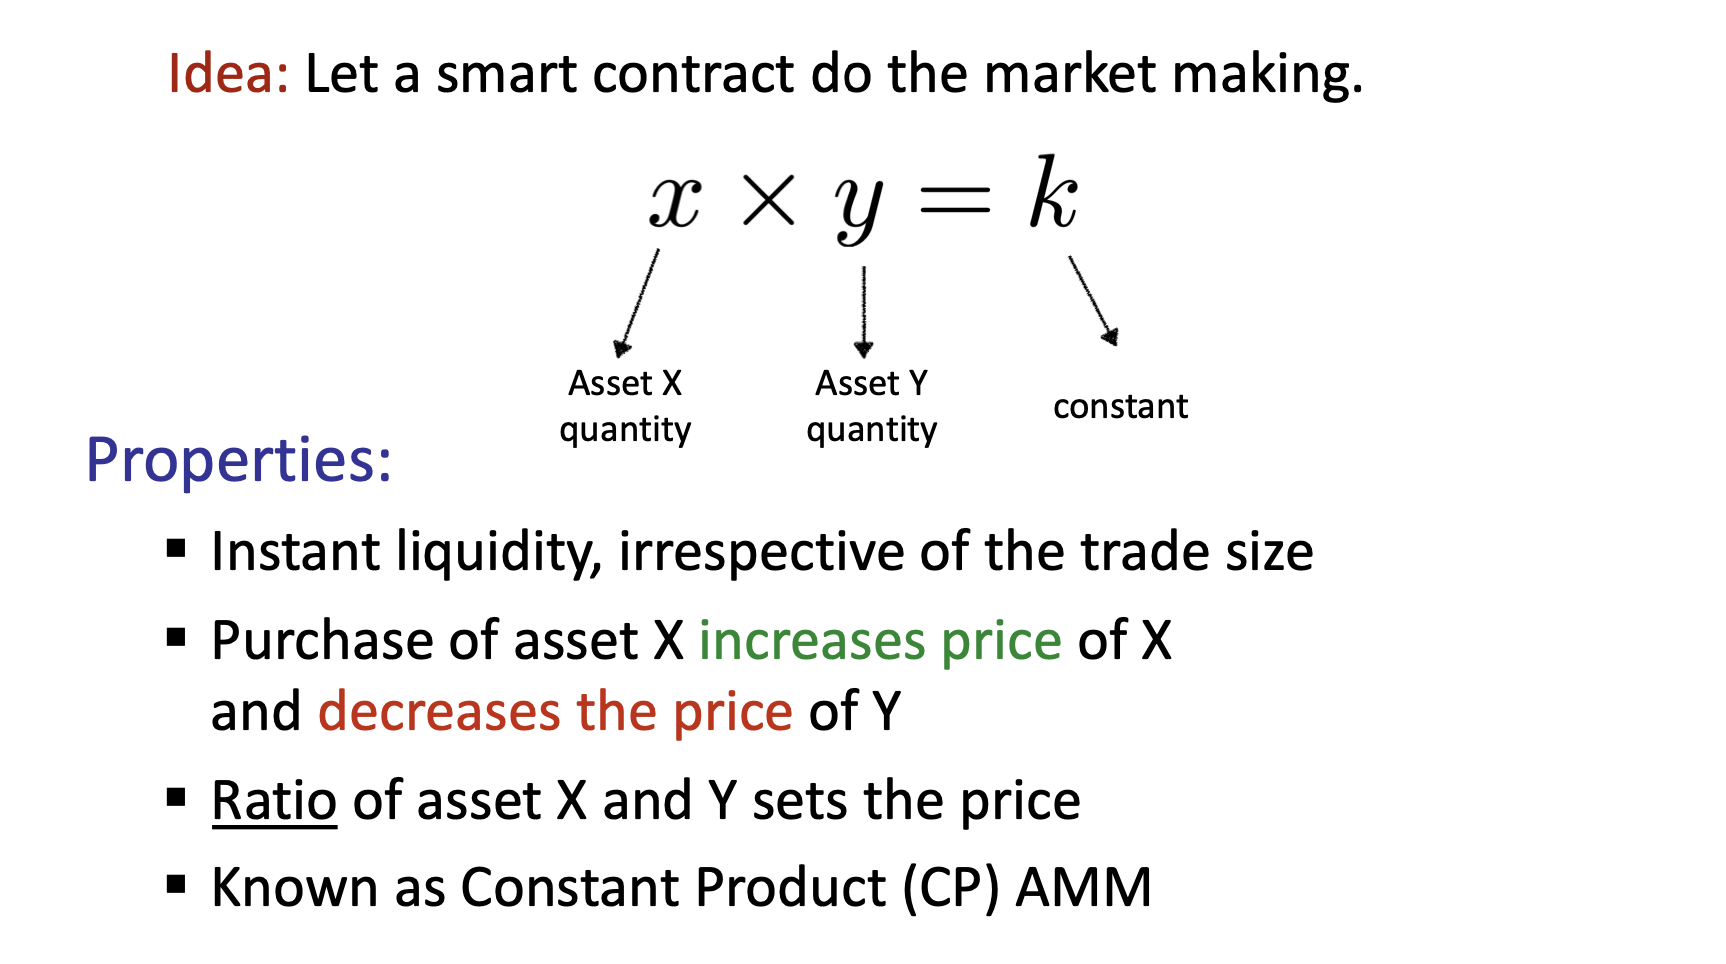
\includegraphics[width=0.5\textwidth]{Bildschirmfoto 2024-04-02 um 15.09.34.png} 
    \caption{Constant Product Formula, \scriptsize{source: lecture 4}}
    \label{fig:DoS-attack}
\end{figure}
\\


%to do :: still have to finish this 
Pro: instant liquidity, don't have to wait for a MATCH, HERE ALWAYS HAVE A MATCH
downside of always matching: price changes, the more i want to buy the higher it is ->smoother than with order books. mORE SENSTIVE TO QUANTITY\\

Automated market makers or as we call the AMM's are algorithms/protocols that make decentralized exchanges (DEXes) simpler and less reliant on third parties. Some well-known examples in the DeFi space that I want to mention are UniSwap and SushiSwap. UniSwap is one of the pioneers in AMM's using smart contracts and liquidity pools. SushiSwap, a DEX based on the UniSwap sourcec code(%idk if we can say source code with these kinda of cthings)

, introduced some extra features to attract more users.  Despite the decentralized nature of AMMs, some centralized elements still remain: For example, when users need to vote on important decisions for an AMM protocol, there must be an organization coordinating these votes. We call these organizations "decentralized autonomous organizations", short DAOs.  They handle and coordinate decisions for various DeFi protocols, such as AMMs and token protocols like ERC-20 which we saw in the lectures.\\
\\
To end this AMM chapter, here is an example of a constant AMM. This may provide a better understanding of how these protocols operate. It's important to know that in AMMs, the tokens involved are typically fungible (see Quiz Chapter for definition). Otherwise, defining an exchange ratio for these currencies becomes way more complex.
\begin{figure}[h]
    \centering
    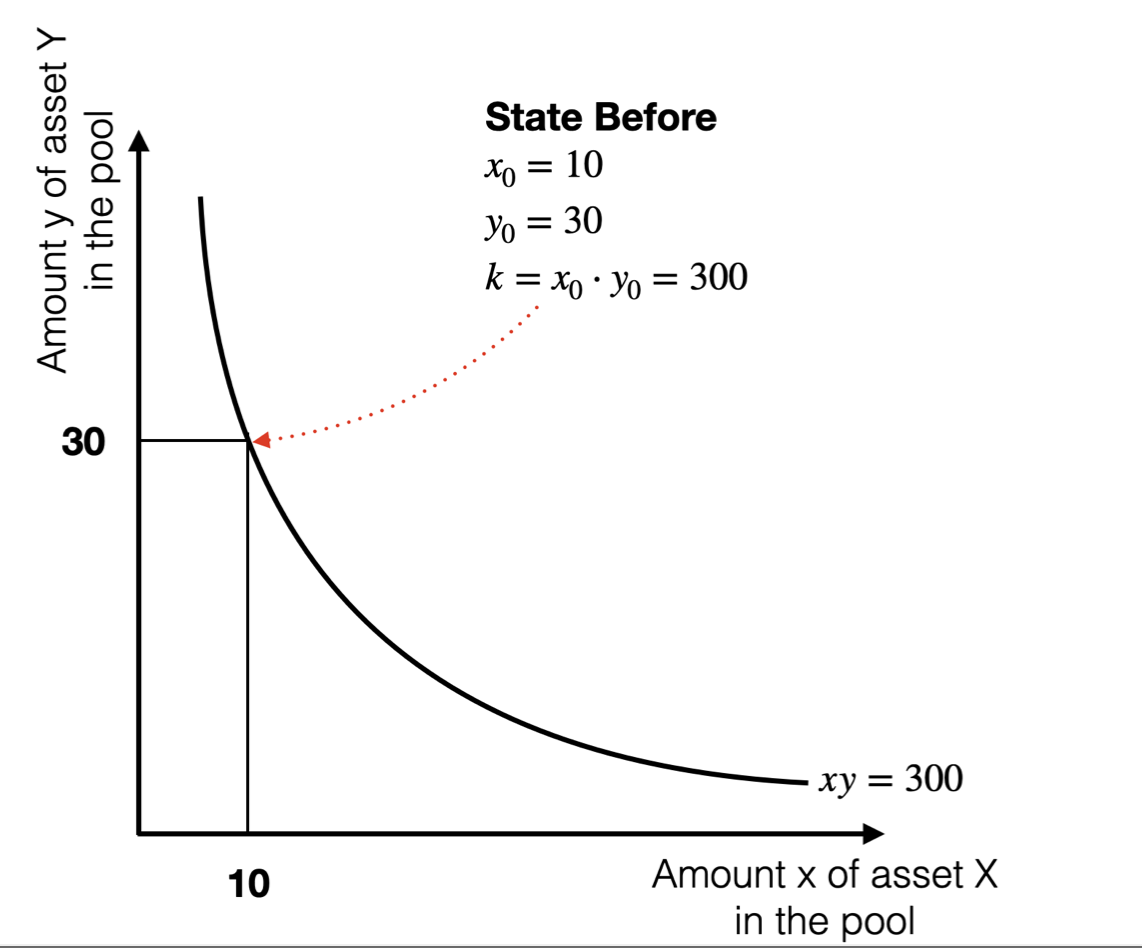
\includegraphics[width=0.5\textwidth]{Bildschirmfoto 2024-04-02 um 15.16.43.png} % Replace 'example-image' with the filename of your image
    \caption{constant AMM, \scriptsize{source: lecture 4}}
    \label{fig:DoS-attack}
\end{figure}
\begin{itemize}
    \item {State before: In the pool are 10 assets of x and 30 assets of the currency y, now if we want to get 10 coins of the assets y, how many coins do we need to provide to the pool?}: 
    \item {As k needs to remain constant, we need to look at the equation and see how the parameters change. As we want to get 10 assets of y, the y amount will drop from 30 to 20 in the pool. Thus the x amount has to increase from 10 to 300/ 20 = 15. Hence we need to put 15-10 = 5 X coins into the pool.}:  
    \item {So if we provide at least 5 coins of X the smart contract is satisfied and we will get 10 coins of Y.}
\item {What happens if we add more liquidity to the pool, hence increase k ? In terms of prices nothing changes, only the constant product k is higher.}
\end{itemize}What we observe with AMM's is that the more we buy from an asset, the more expensive each additional part becomes. This phenomenon is known as \textbf{expected slippage}, which refers to the expected increase or decrease in price based on the trading volume and available liquidity. In simpler terms, buyers may end up paying a higher price for their order than the market price due to a lack of liquidity in the pool. The more liquidity a certain coin has, the less impact a single trade of that coin has on the price.\\
\\
Additionally, there is the concept of \textbf{unexpected slippage}, which occurs when an unexpected purchase of the same asset front runs our trade, hence impacts our price execution. This can result in either a better or unfortunately a worse execution price for us.\\
\\
Now, we can ask ourselves if it's possible to incur a significantly worse price than first stated in the AMM. No, because there is the option to set a maximum slippage that we are willing to accept. If the slippage exceeds this limit, the transaction will fail.\\
\\

\textbf{Advantages of AMM}:
\begin{itemize}
    \item {no order book maintenance}
    \item {simple implementation}

\end{itemize}
\textbf{Disadvantages of AMM}:
\begin{itemize}
    \item {Danger of impermanent loss }: 
    \item {Slippage (especially in low liquidity markets)}: 
    \item {sandwich attacks (just mentioned, didnt cover iin lecture }:  
\end{itemize}
%not sure where to really place this 
\subsection{Impermanent Loss} %have to finish s^this still only notes from lecture yet 
The effect/ loss we encounter through arbitrage. Called impermanent loss, because it is only a loss if we realize it aka withdraw from the pool. Else doesn't encounter the loss. Phenomena in AMM but not in order books.


\subsection{Pegged and Stablecoin AMM} 
In the lecture we encountered different types of Stablecoins: 
\begin{itemize}% to do
    \item {Reserve-based}:For each coin, money is being collaterized in a bank. An example is USDC, for every issued USDC token on the blockchain, there is an equivalent coin in the bank. 
    \item {Collateral based}: Here the idea is to overcollaterize each token. An example for this Stablecoin type would be MakerDAO, i. ex DAI. To retrieve DAI coins, the user has to place an 150\% worth of another assets in a special type of smart contract (see Chapter Liquidations). Collateral based Stablecoins are fully on chain.
    \item {Algorthmic}: Only there existence was mentioned in the lecture. As an example in the lecture they provided the Ampleforth(AMPL) coin.
\end{itemize}Before we look at those in more detail, here a general definition of a Stablecoin: A Stablecoin is a cryptocurrency that maintains a stable ratio/value relative to another currency or just asset in general. The aim of Stablecoins, as the name suggest, is to stabilize the currency, hence avoid high volatility's which f.eg Bitcoin or Ethereum have. So they try to have as little price fluctuations as possible, which is attractive for investors who want less risk i.ex want to avoid the volatility certain other "crypto-assets" have.
In combination with Stablecoins the word  \textbf{"pegged" }often appears. A pegged cryptocurrency refers to a coin whose value is bound aka "pegged" to the value of another asset. Most often this other asset is a fiat currency like the Swiss Franc or resources like gold or silver. In general we would peg a currency to reduce its price volatility. Often the aim of the exchange rate is 1-to-1. To refer to previous sections we can also go back to the notion of slippage with Stablecoins. Stablecoins exhibit a more "linear" swap curve, hence more straight swap curve. This means they have a reduced risk of unexpected high slippage.\\
\\
Here I want to quickly mention that \textbf{Stablecoins and pegged coins} aren't the same thing. While Stablecoins are often pegged to a specific value or asset, not all pegged coins are Stablecoins. Both concepts are very similar, in detail every Stabelcoin is pegged but a pegged coin doesn't have to be a Stabelcoin. Stablecoins are often pegged to a specific asset like gold or a fiat currency, so they are designed to maintain a \textbf{stable relative value} to another asset. On the other hand, pegged coins refer to cryptocurrencies that are tied or pegged to the value of another asset, but not all pegged coins necessarily aim to be stable. So some pegged coins may experience price fluctuations while Stablecoins are always pegged to maintain stability. Here we should also mention that its not always fully 100\% decentralized, as often  third part like a bank or a DeFi App is involved to execute the exchange from the Stablecoin/ pegged coin  to the value its tied to.\\
\\
Some well-known collateral based Stablecoins are USDC and USDT% finish writting about them -> provide some inputthat they are coverd by a banka etc bla bla 
\begin{itemize}
\item {DAI}: One well-known Stablecoin cryptocurrency is DAI as we have seen in the lecture. DAI is pegged to the US Dollar and as it is a Stablecoin (see Stablecoin Chaptre) it is less volatile like Ethereum and usually maintains a stable value. The creater of DAI is MakerDAO, a decentralized autonomous organization on the Ethereum blockchain.DAI is created and managed by MakerDAO, a decentralized autonomous organization built on the Ethereum blockchain. the organization is based on smart contracts and works with collateralized debt positions (CDPs, see next block). Users can place f.eg ETH as collateral in CDPs and generate DAI tokens based on the value of their collateral amount. This process is also known as minting DAI.
\begin{itemize}
\item \textbf{How is DAI maintained stable?}: DAI stays stable through various methods. It relies on overcollateralization and liquidation of undercollateralized CDPs. This means that to obtain DAI, more collateral must be provided than the amount of DAI received (usually 150\% collateral). Moreover, if the value of the collateral drops below a certain threshold, the CDP is automatically liquidated. For instance, if someone's collateral falls below 150\%, MakerDAO will automatically sell their ETH holdings with a 13\% penalty fee. These mechanisms ensure that DAI is backed by secure assets. When users repay their borrowed DAI, the amount of DAI is burned since DAI is only backed by collateral If a users pays back their borrowed/minted DAI's, the amount of DAI gets burned as DAI is only covered by collateral. I would say DAI is pretty popular as it allows investors to hedge against other, more volatile cryptocurrencies but still allows users to have some stability and enjoy the benefits of DeFi. F eg. if you know that the price of Bitcoin might decrease , you could convert some of your Bitcoin into DAI. Since DAI's value is pegged to the US dollar, it's less likely to experience large price fluctuations compared to Bitcoin. So even if Bitcoin falls, the value of the DAI holdings should remain relatively stable. So you hedged against bitcoins volatility with DAI. But lately the DAI interest rates have increased massively, which makes it a more expensive option.
Just for the sake of completeness I want to add another "easy" option to create a Stablecoin: One could just follow another Stablcoin, which means just use a lot of the other non volatile currency as collateral.
\end{itemize}
\begin{itemize}
\item {\textbf{CDP's}, collateralize debt positions}: A collaterzied debt position can be seen as a lock-up contract. It is a smart contract used by DAO's to  allow users to generate currencies like DAI. Users can lock up their assets as collateral in such CDP's and based on how much worth of collateral they put, the users can generate up to a certain amount of f.eg DAI. The generated dai can then be used for various purposes such as trading or repaying other debt positions. If a user wants to retrieve their locked-up collateral, the must repay the generated DAI including an interest rate. After that, the CDP is considered as closed.
\end{itemize}
\end{itemize}
Now the questions is, what happens if a Stablecoin \textbf{de-pegs}, which means on of the coins a Stablecoin is tied to, drops to zero or in general loses a lot of worth. Like in the CeFi systems, a phenomena called "bank run" is observable. In DeFi, instead of a bank run, we see arbitrageurs attempting to exploit price differences by selling the less valuable coin in a stable swap and acquiring the more valuable one. However, this activity can lead to major in-stabilization of the pool, and investors who enter the pool last suffer, lose the most. Additionally, in such scenarios, some pools become blacklisted to avoid the "bank runs" or rather "pool runs". As seen in the censorship chapter, blacklisting a pool effectively restricts any movement of values into and out of the censored address.

\begin{figure}[h]
    \centering
    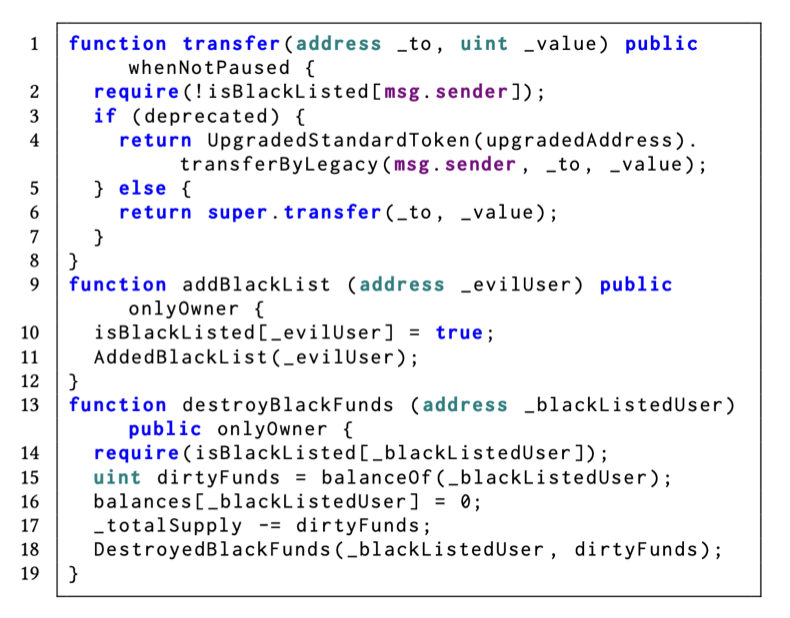
\includegraphics[width=0.5\textwidth]{Bildschirmfoto 2024-04-02 um 16.33.28.png} % Replace 'example-image' with the filename of your image
    \caption{Blacklisting pools, \scriptsize{source: lecture 4}}
    \label{fig:DoS-attack}
\end{figure}

\subsection{Extra: Sandwich Attacks}

Sandwich attacks are attacks where the attackers influence the order of execution to exploit slippage and convexity of the price curve in AMM's. They make use of the order to manipulate the prices: First, the attacker watches the network for a large transaction that will impact the liquidity of a decentralized exchange (DEX). When this transaction is announced, the attacker quickly sends their own transaction to the exchange. The attackers transaction aims to change the price of the assets involved in the big transaction. His transaction will influence the price of the assets in the DEX order book. Once the attacker's transaction is fully executed, the assets price is altered, possibly affecting all the pending transaction that follow. The subsequent transaction, often from a "normal" user, gets executed at the changed price, with the attacker profiting from the altered prices. The name "sandwich" comes from the fact that the user's transaction is sandwiched between the attacker's two transactions, leading to unexpected and unfair price changes. All in all the attacker makes profit from the changes in price caused by its first and then second transaction with the users transaction in between.\\
\\
Sandwich attacks occur when attackers manipulate the order of transaction execution to take advantage of "slippage and convexity of the price curve" of Automated Market Makers (AMMs). The procedure of a Sandwich Attacker : Initially, the attacker monitors the network for a significant transaction that will impact the liquidity of a decentralized exchange (DEX). This means he watches the network for a very large transaction.  Upon spotting such a transaction, the attacker quickly initiates their own transaction to the exchange. This transaction will influence the price of the assets involved in the large transaction. (Think of order book depth and the AMM constant product formula) Consequently, the price of these assets in the DEX order book is affected by the attacker's transaction. Once the attacker's transaction is fully executed, the price of the assets changes, potentially impacting all subsequent pending transactions. The transaction subsequent to the attackers transaction, often from a "normal" user, gets executed at the changed price, with the attacker profiting from the altered prices. The name "sandwich" comes from the fact that the user's transaction is sandwiched between the attacker's two transactions, leading to unexpected and unfair price changes. All in all the attacker makes profit from the changes in price caused by its first and then second transaction with the users transaction caught in between.\\ 
\\
Now, one might ask: How does the attacker even know that the victim's transaction might be executed and placed in a block on the blockchain soon? Since we are in a blockchain-based system like Ethereum, all transactions are broadcasted to the entire network. Every participant, including the malicious attacker, is informed about all transactions.\\
\\
To avoid such unfair attacks like the Sandwich Attack DEXes have different attempts to especially avoid these front-running transactions (the attackers transaction being placed prior to the users transaction). They tried to implement increasing transaction fees or in general tried to improve transaction processing such that there is no time to issue another transaction beforehand. There are also notions where the execution order gets fixed before the content of each transaction is revealed. Disabling the attacker to spot large transactions. In the next subsection some protection mechanism against Sandwich Attacks are presented:\\

\begin{figure}[htbp]
    \centering
    \begin{subfigure}[b]{0.4\textwidth}
        \centering
        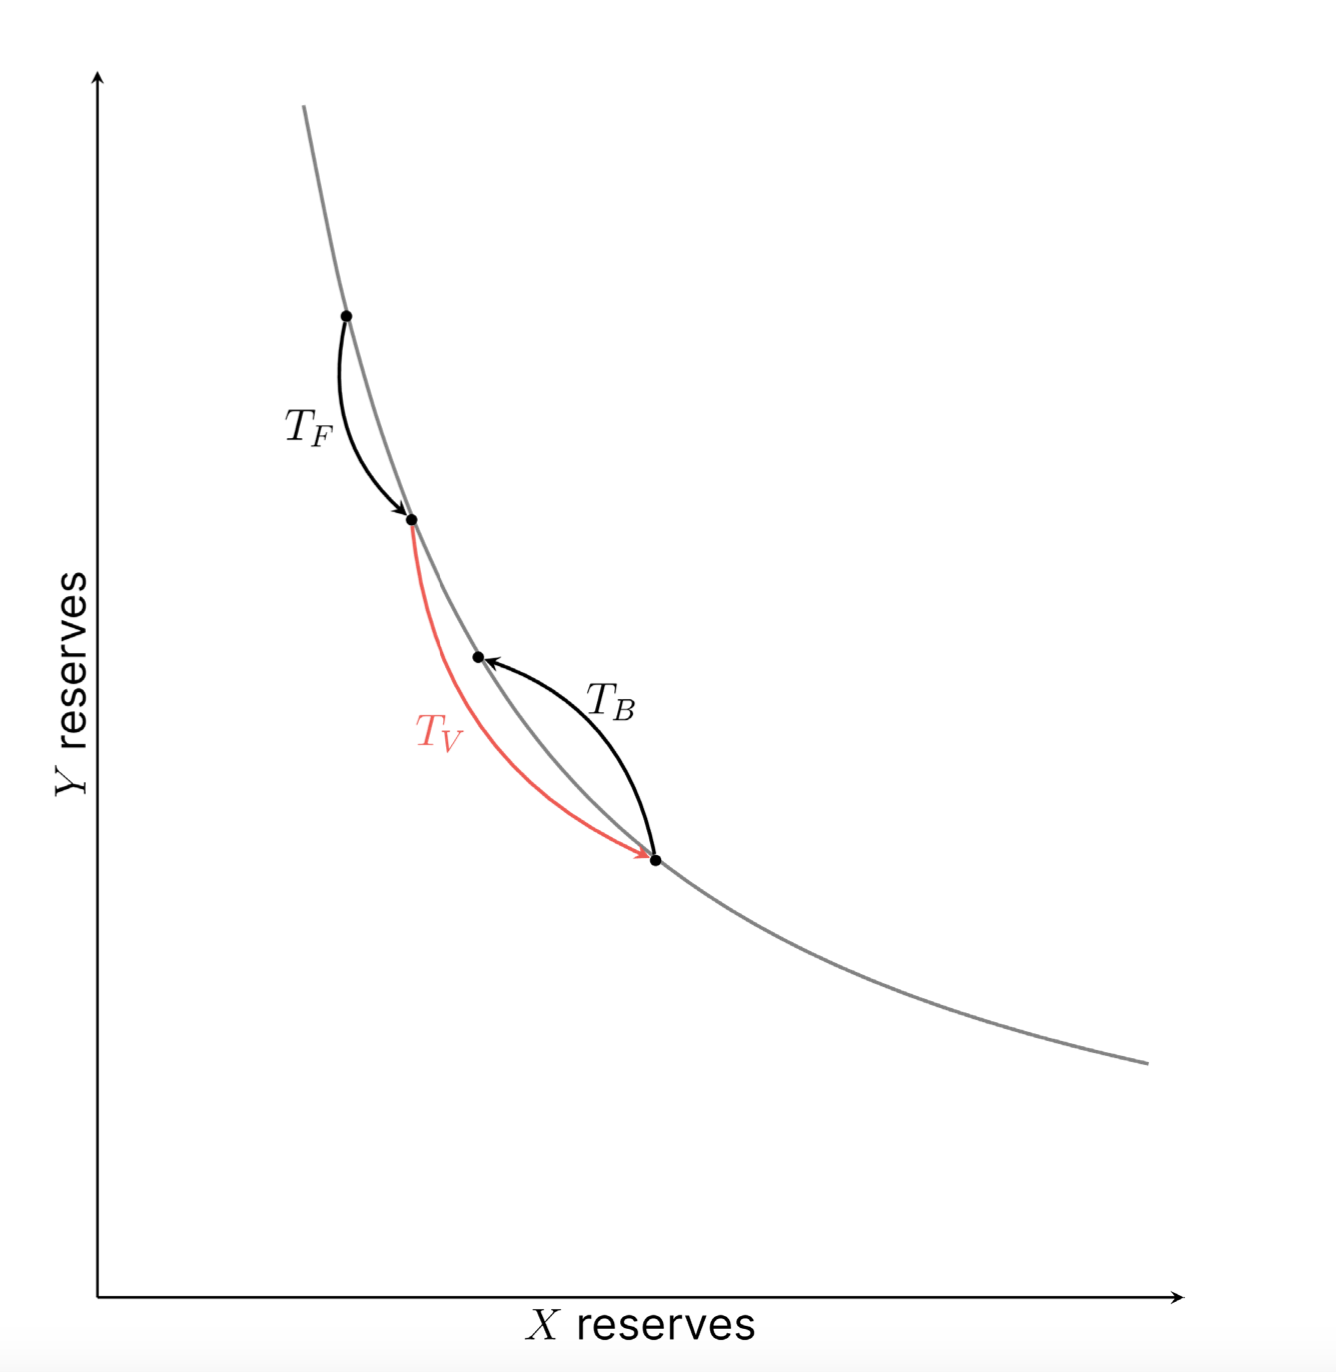
\includegraphics[width=\textwidth]{Bildschirmfoto 2024-04-02 um 16.56.24.png}
        \caption{Sandwich Attack Mechanism}
        \label{fig:img1}
    \end{subfigure}
    \hfill
    \begin{subfigure}[b]{0.4\textwidth}
        \centering
        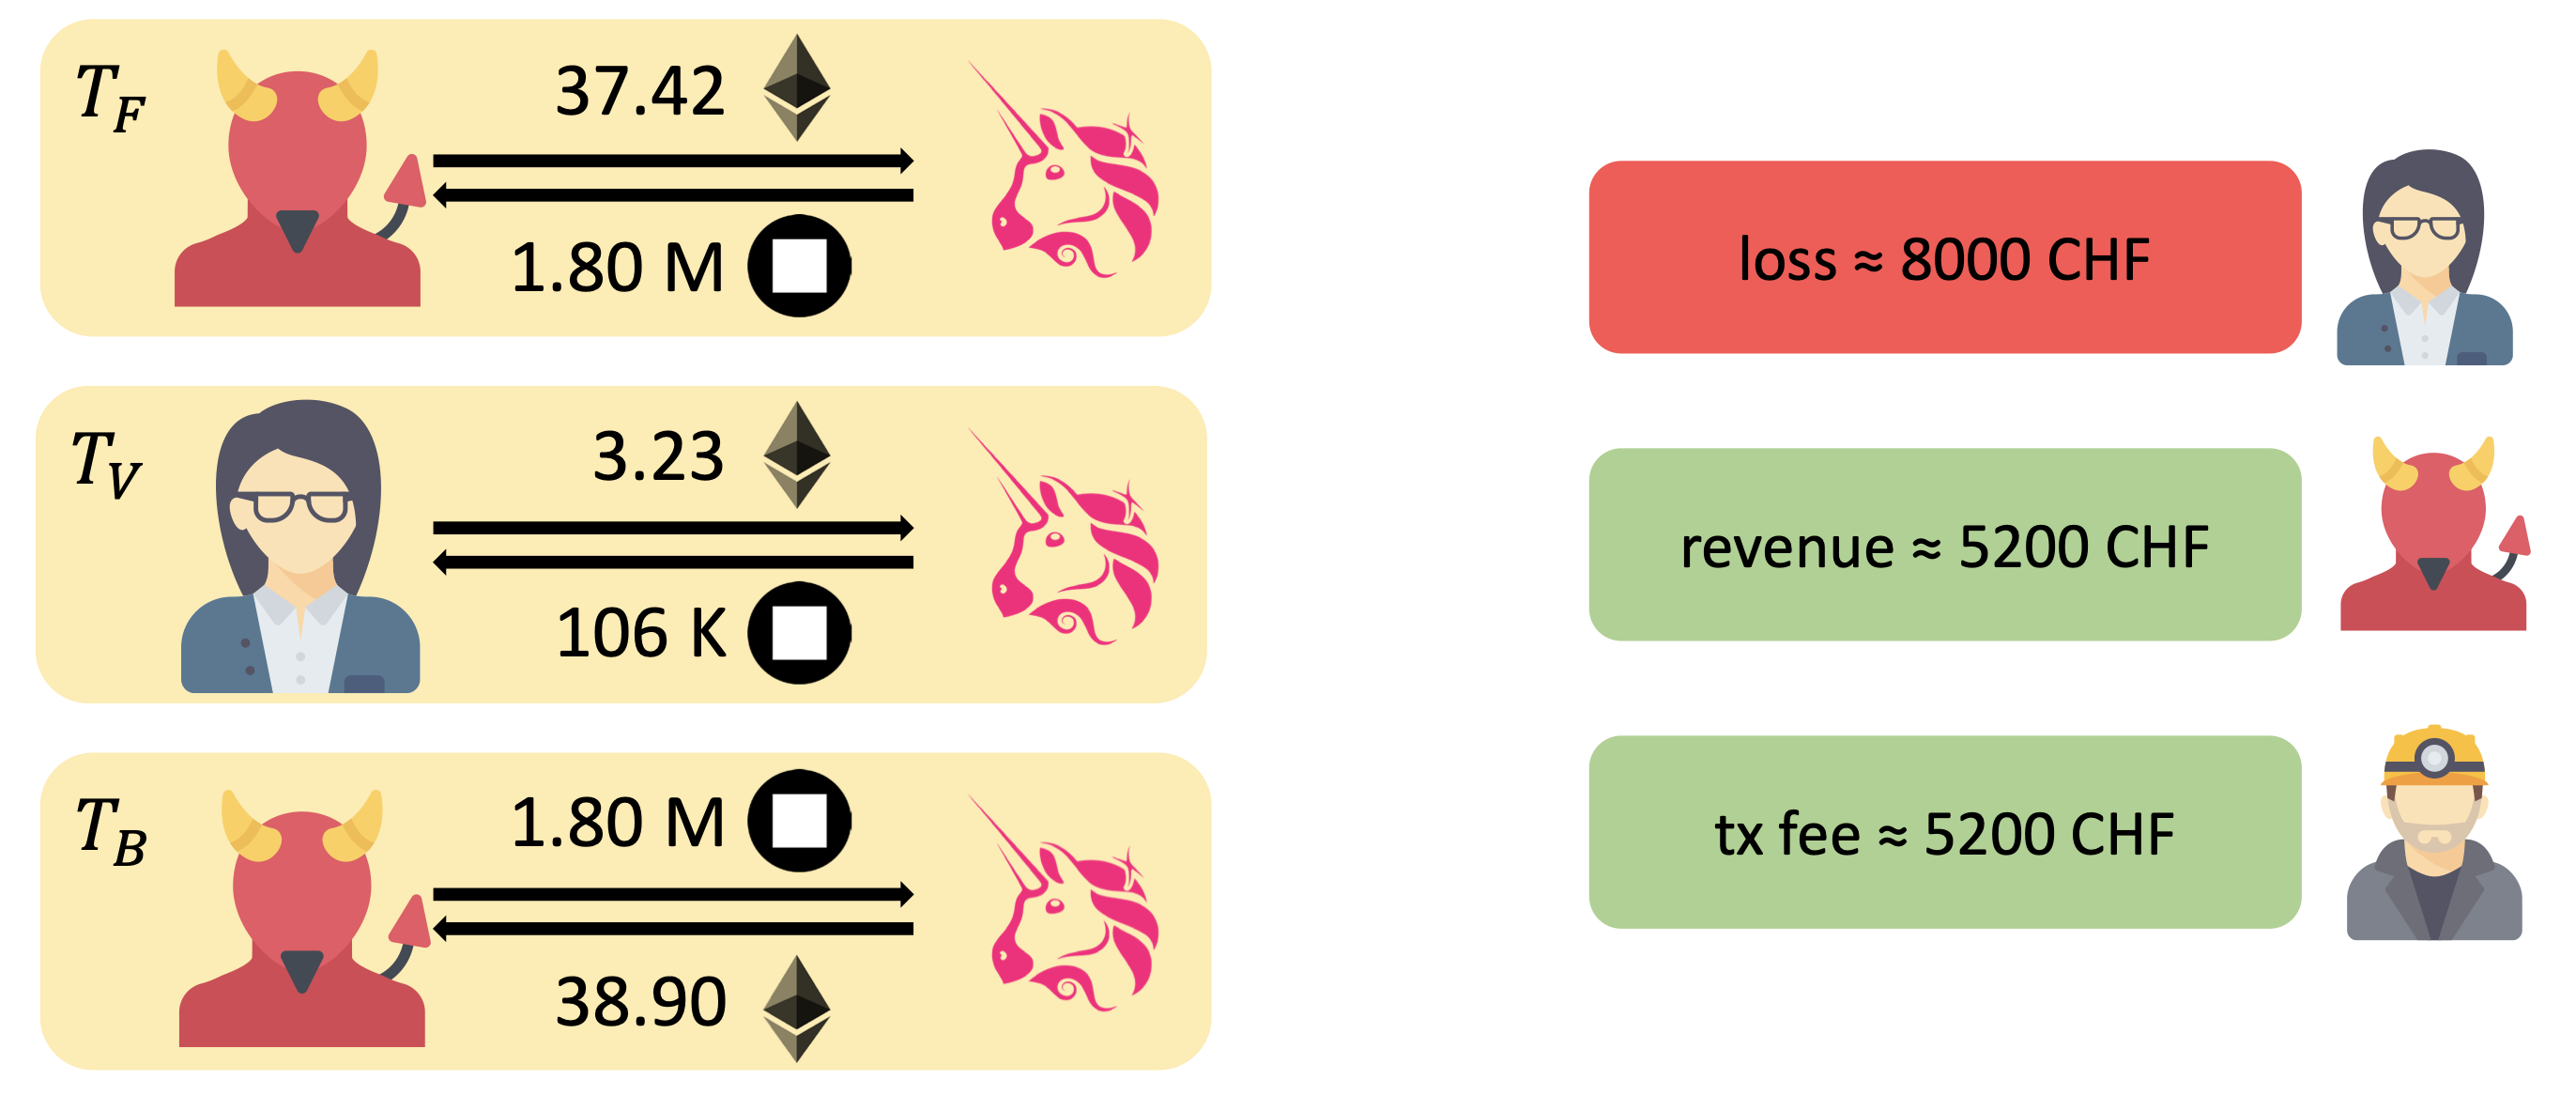
\includegraphics[width=\textwidth]{Bildschirmfoto 2024-04-02 um 16.56.55.png}
        \caption{Sandwich Attack Prevalence}
        \label{fig:img2}
    \end{subfigure}
    \label{fig:both}
\end{figure}

\textbf{Protection Against Sandwich Attacks}

\begin{itemize}
\item {Slippage protection}: One option is to directly encode into the transaction what maximum percentage of slippage we tolerate. if this slippage level is over-shooted the transaction will not be executed. This form of protection is simple to implement but is rather handling the symptoms of sandwich attacks rather than disabling  the attacks themselves.
\item {Third Party Ordering}: We could let a trusted third party order the transactions. This then should happen in a manner such that the third party isn't biased towards to the attacker. To avoid a malicious third party, trust is the key and decentralization focuses on avoiding the need of trusted third parties. In general, letting a third party to be involved is an efficient approach but contradicts the concept of decentralization.
\item {Committee Ordering}: Very similar to third party ordering, committee ordering involves  a whole committee of trusted third parties. With some consensus mechanism they agree on how to order the transactions. In committee ordering the influence of a malicious third parties is little but we encounter problems if they are multiple. Again this approach is relatively fair and efficient but still reduces decentralization.
\item {Commit and Reveal}: This approach executes in two phases. First the committed transaction get encrypted and an ordering on them is imposed. Only after their execution order is fixed, the transaction contents get revealed. Hence an attacker doesn't have access to a transactions content/amount until the order is fixed. This is a quite secure option but come with high costs and increases latency.
\item {First come, First serve}:
The "First Come, First Serve" rule can be seen like the standing in line at a store. Whoever gets there first gets the help first. For DEXes it means that transactions are handled in the order they're received. This helps stop sandwich attacks as DEXs prioritize the execution of transactions based on their arrival time. Thus an attacker cannot squeeze in a malicious transactions, if the users transaction was issued first.So this approach makes it less likely that attackers can exploit the order of transaction execution and manipulate prices to finally profit from the market.
\end{itemize}


%guest speech content 

\section{Guest Speech Content}

\subsection{Lecture 4: DeFi leverage }

In the first half of the lecture the professor introduced the concept of flash loans, leverage and arbitrage. Then a presentation about DeFi leverage presented by BIS, the Bank for International Settlements , followed. In this chapter I will just quickly cover the key points and definitions. 
\begin{itemize}

% to do , wrote that done during lecture but dont remember anymore.

\item {Volatile and Stable Coins}: As we have previously seen a Stablecoin is a coin that tries to  maintain its value by pegging its price to a stable assets like a fiat currency. Volatile coins as the name suggests are more volatile, hence have a lot of price fluctuations and are not stabilized by any other asset.

\item {Leverage}: In very simple terms leverage describes using borrowed money to invest, to amplify the returns on an investment by using debt. In German on often refers to leverage as some sort of "Hebelwirkung". 


\item {Delaveraging, False Delaveraging }: Deleveraging refers to an borrower paying down his debt or at least parts of it. So deleveraging is a synonym to "reducing the amount of debt one owns". So the goal is to reduce its own overall debt burden.\\
\\
False Delavering refers to a situation where an actor delavrages even though the reduction of debt levels in not healthy nor sustainable. We talk about delaveraging when actors manipulate their financial situation to make it appear as though they are reducing debt when they aren't. False deleveraging creates the illusion of financial health of an actor and hides his actually debt level.
possible ways to false deleverage is just hiding debt position or as we say in german "abschreiben", which means putting them on an off-balance sheet 

\item {Closed factor}: Refers to the maximum proportion of the debt that can be repaid in a liquidation. The close factor is a metric to measure the liquidity of an asset. If is usually calculated based on the trading activity of that position.A high closed factor suggests that the security is rather illiquid because it frequently goes without any trading activity. A small closed factor indicates that the security is liquid, as it has a trading activity on several days within the choosen time period.

\item {Shorting and Longing: }: Shorting and longing are both actually trading strategies often seen on the stock market. They make use either of falling or increasing asset prices. They are based on different believes on how the assets prive will evolve. Short selling (shorting) is known as borrowing a certain assets from a lender and selling it on the market to someone else, hoping the after you sold it, the price will fall. Then after the price has fallen the next step in shorting would be to buy the asset back, but at the new, lower price. Finally you would return it to the lender with a difference as profit. Base idea of shorting is gambling that the asset price will fall.//
//
Longing is the more intuitive trading strategy where you bet on the assets prices going up. First one would invest in an asset where you expect that its price will increase over time. "Going long" means buying an assets and keeping it with the belief that its value will increase such that you will sell it at a future point in time. When you sell it later you you expect that it price will be higher to make a profit. Here I really want to mention that shorting and longing are strategies on how investors choose to invest their money, so it refers to what investors think and expect but not what has to happen.

\item {Negative correlation}: Is a term that is also often used outside of the Finance World and refers to two or more parameters moving in the opposite direction. In DeFi negative correlation can be a trading/ investment strategy to diversify its portfolio. If two assets are negatively correlated, the price of of one assets goes up while the price of the other asset has the tendency to go down. So an investor can use this to offset potential loses and reduce his total risk. In the previous paragraph we saw shorting and longing : For example if an investor makes a short selling (decrease in asset value) , he may also seek another asset which has a negative correlation with it, hence an expected price increase. That way, if the first asset's price does indeed fall, the second asset's price is likely to rise, so he could compensate any potential loss from the short. All in all in finance negative correlation is a tool to optimize the portfolio by better managing risks.


\item {Pooling collateral}: 
Pooling collateral refers to  combining securities/collaterals (f.eg a house, other assets etc) into a single pool to secure a loan. The borrowers put their collateral into a shared pool, which is then used as security for the entire group of investors. Out of CeFi perspective this is very unusual as a lender has no real guarantee about the security of his loan. In DeFi it happens that lender take the good securities out of the pool and trade it against the less secure ones. An option to execute such a trade is with a flash loan, % review this, not sure if happy about it

\item {Fixed Spread Liquidation Strategy}:
Is a way how an  investors can manage its risks. In this approach the trader sets a predefined price level at which he will automatically exit the market, to limit a potential loss and at least secure some profit. For this the trader fixes a price spread, therefore the name, between his entry price (price he bought the assets) and the liquidation price (price at which he decides to sell to minimize the loss). Selling the assets and therefore exiting the market is often refereed to as "closing the position".

\item {Bad debt}: We consider a position as a bad debt if its financially rationale neither for the borrower nor the lending platform to close the position. Often it refers to money that is owed to a lender but is unlikely to be recovered because the borrower is financially unable to refinance it
\end{itemize}

Conclusion of the speech: %still open  !!!!!!!!!!!!!!!!!!!!!!!!!!!!!!!!!!!!!!!!!!!!!!!
one unique feature of DeFi, when borrower a loan -> pooled together with other collateral's, don't really know by what collateral I'm backed up by. Can use flash loans to do collateral swap and leaf unsafe collateral in the behind.


\section{Quiz Content}
Here is a collection of terms, questions and topics covered in the lecture quizzes. I tried to structure them according to topic.
\begin{itemize}
    
    \item \textbf{Financial Inclusion}: Refers to accessibility and availability of financial services to actors, especially in under-served communities. All parts of society should have access to a range of affordable financial services like bank accounts, investment opportunities and credit services. Financial education is an additional important aspect of financial inclusion. 
    (taken from lecture slides)
    
    \item \textbf{Collateral}:  Assets that a borrower pledges to a lender to secure a loan.
    If the borrow can't repay the loan, the lender will become owner of the collateral to recover the outstanding debt.
    
    
    \item \textbf{Over-collateralization}: Refers to pledging more assets than required by the collateral requirements. If the requirements says 150\%, the borrower would have to provide collateral worth 150\% of the loan amount. Any collateral valued more than those 150\% would refer to over-collaterizing.\\
    Benefits of over-collaterization is
    
    \begin{itemize}
     \item {Risk reduction}:
        Having more collateral provides an extra protection for the lender, hence reduces his risk in case of loss.  
    
    \item {Market volatility protection}:
    As with over-collaterization the lender has more protection also against market volatility's. Stock prices and in general the value of assets fluctuates, with a over collaterized loan, the lender has a buffer against these ups and downs.
     \end{itemize}

     
     \item \textbf{Market Makers}: :
        Market makers are individuals or entities that are like the backbone of a market. They make it easier for people to trade, set prices, and keep things running smoothly. They constantly buy and sell stocks, bonds etc. to publicly stated prices and in that way ensure a liquid market. They kinda ensure that there is always a counter party if a trader wants to transact.
    
    \item \textbf{Bid-Ask-Spread}: Difference between the buying (bid) and the selling prices (ask). The goal is to buy at low prices and sell for a high prices. The difference is then called the spread and is a compensation for having provided liquidity to the market.
        
    \item \textbf{Transparency}: Transparency is a big keyword in DeFi. Technologies such as blockchain are called transparent as they allow each user to see and trace every transaction in the system. For some this transparency property enhances trust for the DeFi system.

    
     \item \textbf{Financial Empowerment}: DeFi promises to empower the individuals by giving them more control and access over their assets. In DeFi the user often have a so called private key which allows them to directly engage in financial exchanges etc, without needing a traditional intermediaries.
    
    \item \textbf{Value at Risk aka "VaR"}: Is a statistical measure and describes the potential loss of an investment monitored over a time interval. VaR refer to an investment and a certain confidence level and estimate the maximum loss an investment is likely to incur with this confidence level.\\
    For example, a 95\% VaR of \$1 million over one week means that there is a 95\% probability that the portfolio will not lose more than \$1 million over the next week.

    \item \textbf{Excpected shortfall aka CVaR}:
    Also known as Conditional Value at Risk (CVaR), is a risk measure that stands for the average loss that would occur beyond the VaR threshold. It represents the expected value of losses exceeding the VaR level.  

    \item \textbf{ERC-20}: ERC20 is a token-management contract for Ethereum-based tokens. This means it's a set of rules and guidelines i.ex like an interface for tokens. The characteristics of such ERC-20 tokens are that they are fungible aka every token is identical to every other ERC-20 token, which is a useful characteristics in DeFi applications. This is of importance because they can be exchanged in a 1-to-1 ratio. ERC-20 has become the most used standard for tokens on the Ethereum blockchain.
    (Btw ERC stands for "Ethereum Request For Comments and mirrors how protocols and standards are discussed and developed within the Ethereum community. Each users can review and take part in discussion about these suggested standards before they actually get implemented). 

    \item \textbf{ERC-721}: As ERC-20 is a used standart for fungiable tokens, ERC-721 is a standard predominantly used for Non-fungible tokens (NFTs) in Ethereum. It represents a set of rules and guidelines for representing ownership of NFT's. Each token created using the ERC-721 standard is distinct from every other token, hence they are non-fungible as each token has unique properties. This implies that they aren't exchanged on a 1-to-1 basis.

    \item \textbf{Miners}: Miners are essential actors in the Ethereum network. They are responsible for including transactions into a block and creating new blocks. First Miners include pending transactions into blocks. Whenever a user wants to do a transaction (f. eg sending ETH to interact with a smart contract), it goes into the network and  miners will pick it up to process. The decision which miners can create the new block, the different miners compete to solve a puzzle. This process is computationally intensive. When a miner has successfully solved the challenge he can create and provide the new block. For their efforts miners get newly created ETH (for each successfully mined block). Additionally they can also have to transaction fees within the block they mined.

    \item \textbf{Transaction fees}:
    These are fees paid by users to miners to prioritize their transactions and ensure rapid of their transaction by miners.

    \item \textbf{Block generation}: It describes the process of creating new blocks and adding them to the blockchain. It is done by the miners in a blockchain network. First there has to be a collection of transactions waiting to be executed aka waiting to be in a block. Then the mining starts which means that miners compete in solving a puzzle, the first miner to solve it can create the new block and add it to the chain.

    \item \textbf {Liability}:  In DeFi liability refers to the responsibility that actors or whole institutions have in case something goes wrong with a DeFi item like a protocol or a whole platform. Unlike in traditional finance where it is more clear that liability is assigned to the centralized entities like banks, determining the liability in DeFi strucutres is way harder. As Ethereum operates on blockchain technology with smart contracts etc. there is no central authority to hold accountable, instead in DeFi it depends on different factors like protocol type, the actions of each users etc. Overall addressing liability in DeFi is less obvious and I think as DeFi continues to evolve, liability is one of the concerns that need to be tackled, especially if one wants ensure stability of these financial systems. In german liability refers to the term "Haftung".

    
    
volatile coins vs stable coins -> can level up using the borrowed sc to buy more vc, can level up exposure to a volatile coin,

% work in progress, this is all still open.
\item \textbf{Anonymity Set}:Is the amount of deposits in a Tornado Cash pool. Refers to the level of privacy. F.eg a Tornado Cash pool with 1000 deposits has a anonymity set size of 1000 and a privacy level of 1/1000.

\item \textbf{Anonymity Set}:Is the amount of deposits in a Tornado Cash pool. Refers to the level of privacy. F.eg a Tornado Cash pool with 1000 deposits has a anonymity set size of 1000 and a privacy level of 1/1000.

\item \textbf{Under-Collateralization}: Undercollaterization: such protocols exist, money that we get is tied to a specify purpose, doesn't happen often -> mostly in the over-collaterized part 

\item \textbf{Health Factor}: Health Factor: 
    (Sum of:  value of collateral x liquidation threshold )/ total value of debts
    if becomes bellow one, position might become liquidated

\item \textbf{Borrowing Capacity}: borrowing capacity

\item \textbf{Base APY, Reward APY}:
 Reward APY paid by the borrower.
 
\item \textbf{Leverage}: Leverage : bet in a certain direction

\item \textbf{Liquidation Spread}:liquidation spread: motivation why liquidator would do something,
"bonus or discount" that a liquidator can collect when liquidating collateral.

\item \textbf{Arbitrage}:


\item \textbf{Liquidity Pools}:

\item \textbf{LP Tokens}:LP Tokens ->can get her thigs out of the pool by provding the LP tokens (are usually fungible)

\item \textbf{Flash Loan}: The concept of a flash loan is guaranting a loan to a borrower without the risk of defaulting on the debt, in a single atomic transaction -> intrest ratoe of 0.3 /0.4 \% . Only possible because we can have multiple actions in one transaction. 
What if we lose all the money we had in a flash loan ?  Can include assertions in the transaction such that if both assertions fail, the transaction will not be executed.
When can a flash loan fail ?
When we have unexpected slippage, our assumption of the arbitrage transaction fails because someone else placed their transaction before us.
Do we have a concept of time in the blockchain i.ex block execution ?
Flash Loan Use Cases: 
    (risk-free) arbitrage, wash trading
how to use flash loans in sandwich attacks ?
What about the transaction fees for a flash loan ? Transaction fees for flash loans are relative small f.eg a transaction fee for a flash loan can be in the order of 100 USD even if the loan amount can grow beyond 1B USD (source :: Quiz lecture 5)

depeg/pegged coins

\item \textbf{LP Tokens}:



\end{itemize}

\section{Liquidations}

\section{Liquidations In Traditional Finance}
in defi way way faster, dai is minted out of thin air -> gets created out of the smart contract, 
fixed spread liquidation: liquidator repays debt of borrowing position and acquire the collateral at a discounted price from the position in return (he repays the debt and can acquire the collateral in return)
why is there a discount ? as inscentives, fixed spread in liquidation is the fixed discount i get, -> can be completed in one transaction, need on-chain price oracles to know that price changed >>( can use on chain or off chain oracle),

closed factor 

auction liquidations: liquidators bod over time until the auction terminates, requires multiple blockchsin transaction,
MakerDAO was working like that, to more competition between the liquidators, the less spread a liquidaotr will make, market force will determine the price, but takes longer, more overhead on the blockchain hence more transaction fees for everyone.

market bot failure: was  amrket collpase, decreaseof prices, and as everyone started to panick -> gas fees aka transaction started to rise ->more liqiudation opportunites -> Maker DAO Bot issued but these transaction werent executedd ? why : because of to low gas fees they were not mined, were not porgrammed for such cases  -> google why 8 million could be taken for 0 DAI.Important hwen writing a Bot need to consider extrem cases.

what if sudenly a lot of collateral becomes liquidatable ? good opportunity for liqudators, can make mone but liquidator get those assets and will sell it one the market and then the asset price decreases which in turn makes more positons liquidable if they are coverd with that decreasing asset  -> "negative cycle"

flash loan based liquiation :which liquidations work in a single transaction ? the makerDAO tent and bent option and fixed spread option 

bad debt: if none will buy the collteral anymore aka the price is to bad -> bad debt, extra afety messure like extra coin pools to repay bad debt but bad debt is realstic scenario, 

 what if i want ot be liquidator but don't have enough money to upfront repay ? can do a flash loan based liquidation, only works if liquidation completes in one transaction --> see above but have 3 types of fees : on flash loan, on liquidation and transactions 

 collateral swap:
change debt postions -> from ether colltaeral but another currency as collateral here USDC -> all done in one transaction.

but why would we do that ? if we know that a certain price will drop and i dont want to be liquidated ->swap my collateral to another collateral.

optimal to do 2 sucesiv liquidations -> can liquidate until position is almost helathy but not yet and then liquiate another one. -> why is this good ?

exogenous vs endogenous variable : outside vs inside force, determined outside vs inside the model f.eg in makerDAO assets price is exogenous akaa independent of makerDAO system,
endogenous variable -> inside the model, 


stability meassures: relative metric -> volatility or standart deviation of returns or maybe worst drop over a timeframe, 



why could a transaction 

maker dao websites, defi lama etc.

\section{DeFi Glossary}
 
\end{document}